% Options for packages loaded elsewhere
\PassOptionsToPackage{unicode}{hyperref}
\PassOptionsToPackage{hyphens}{url}
%
\documentclass[
  doc,floatsintext]{apa6}
\usepackage{amsmath,amssymb}
\usepackage{iftex}
\ifPDFTeX
  \usepackage[T1]{fontenc}
  \usepackage[utf8]{inputenc}
  \usepackage{textcomp} % provide euro and other symbols
\else % if luatex or xetex
  \usepackage{unicode-math} % this also loads fontspec
  \defaultfontfeatures{Scale=MatchLowercase}
  \defaultfontfeatures[\rmfamily]{Ligatures=TeX,Scale=1}
\fi
\usepackage{lmodern}
\ifPDFTeX\else
  % xetex/luatex font selection
\fi
% Use upquote if available, for straight quotes in verbatim environments
\IfFileExists{upquote.sty}{\usepackage{upquote}}{}
\IfFileExists{microtype.sty}{% use microtype if available
  \usepackage[]{microtype}
  \UseMicrotypeSet[protrusion]{basicmath} % disable protrusion for tt fonts
}{}
\makeatletter
\@ifundefined{KOMAClassName}{% if non-KOMA class
  \IfFileExists{parskip.sty}{%
    \usepackage{parskip}
  }{% else
    \setlength{\parindent}{0pt}
    \setlength{\parskip}{6pt plus 2pt minus 1pt}}
}{% if KOMA class
  \KOMAoptions{parskip=half}}
\makeatother
\usepackage{xcolor}
\usepackage{color}
\usepackage{fancyvrb}
\newcommand{\VerbBar}{|}
\newcommand{\VERB}{\Verb[commandchars=\\\{\}]}
\DefineVerbatimEnvironment{Highlighting}{Verbatim}{commandchars=\\\{\}}
% Add ',fontsize=\small' for more characters per line
\usepackage{framed}
\definecolor{shadecolor}{RGB}{248,248,248}
\newenvironment{Shaded}{\begin{snugshade}}{\end{snugshade}}
\newcommand{\AlertTok}[1]{\textcolor[rgb]{0.94,0.16,0.16}{#1}}
\newcommand{\AnnotationTok}[1]{\textcolor[rgb]{0.56,0.35,0.01}{\textbf{\textit{#1}}}}
\newcommand{\AttributeTok}[1]{\textcolor[rgb]{0.13,0.29,0.53}{#1}}
\newcommand{\BaseNTok}[1]{\textcolor[rgb]{0.00,0.00,0.81}{#1}}
\newcommand{\BuiltInTok}[1]{#1}
\newcommand{\CharTok}[1]{\textcolor[rgb]{0.31,0.60,0.02}{#1}}
\newcommand{\CommentTok}[1]{\textcolor[rgb]{0.56,0.35,0.01}{\textit{#1}}}
\newcommand{\CommentVarTok}[1]{\textcolor[rgb]{0.56,0.35,0.01}{\textbf{\textit{#1}}}}
\newcommand{\ConstantTok}[1]{\textcolor[rgb]{0.56,0.35,0.01}{#1}}
\newcommand{\ControlFlowTok}[1]{\textcolor[rgb]{0.13,0.29,0.53}{\textbf{#1}}}
\newcommand{\DataTypeTok}[1]{\textcolor[rgb]{0.13,0.29,0.53}{#1}}
\newcommand{\DecValTok}[1]{\textcolor[rgb]{0.00,0.00,0.81}{#1}}
\newcommand{\DocumentationTok}[1]{\textcolor[rgb]{0.56,0.35,0.01}{\textbf{\textit{#1}}}}
\newcommand{\ErrorTok}[1]{\textcolor[rgb]{0.64,0.00,0.00}{\textbf{#1}}}
\newcommand{\ExtensionTok}[1]{#1}
\newcommand{\FloatTok}[1]{\textcolor[rgb]{0.00,0.00,0.81}{#1}}
\newcommand{\FunctionTok}[1]{\textcolor[rgb]{0.13,0.29,0.53}{\textbf{#1}}}
\newcommand{\ImportTok}[1]{#1}
\newcommand{\InformationTok}[1]{\textcolor[rgb]{0.56,0.35,0.01}{\textbf{\textit{#1}}}}
\newcommand{\KeywordTok}[1]{\textcolor[rgb]{0.13,0.29,0.53}{\textbf{#1}}}
\newcommand{\NormalTok}[1]{#1}
\newcommand{\OperatorTok}[1]{\textcolor[rgb]{0.81,0.36,0.00}{\textbf{#1}}}
\newcommand{\OtherTok}[1]{\textcolor[rgb]{0.56,0.35,0.01}{#1}}
\newcommand{\PreprocessorTok}[1]{\textcolor[rgb]{0.56,0.35,0.01}{\textit{#1}}}
\newcommand{\RegionMarkerTok}[1]{#1}
\newcommand{\SpecialCharTok}[1]{\textcolor[rgb]{0.81,0.36,0.00}{\textbf{#1}}}
\newcommand{\SpecialStringTok}[1]{\textcolor[rgb]{0.31,0.60,0.02}{#1}}
\newcommand{\StringTok}[1]{\textcolor[rgb]{0.31,0.60,0.02}{#1}}
\newcommand{\VariableTok}[1]{\textcolor[rgb]{0.00,0.00,0.00}{#1}}
\newcommand{\VerbatimStringTok}[1]{\textcolor[rgb]{0.31,0.60,0.02}{#1}}
\newcommand{\WarningTok}[1]{\textcolor[rgb]{0.56,0.35,0.01}{\textbf{\textit{#1}}}}
\usepackage{graphicx}
\makeatletter
\def\maxwidth{\ifdim\Gin@nat@width>\linewidth\linewidth\else\Gin@nat@width\fi}
\def\maxheight{\ifdim\Gin@nat@height>\textheight\textheight\else\Gin@nat@height\fi}
\makeatother
% Scale images if necessary, so that they will not overflow the page
% margins by default, and it is still possible to overwrite the defaults
% using explicit options in \includegraphics[width, height, ...]{}
\setkeys{Gin}{width=\maxwidth,height=\maxheight,keepaspectratio}
% Set default figure placement to htbp
\makeatletter
\def\fps@figure{htbp}
\makeatother
\setlength{\emergencystretch}{3em} % prevent overfull lines
\providecommand{\tightlist}{%
  \setlength{\itemsep}{0pt}\setlength{\parskip}{0pt}}
\setcounter{secnumdepth}{5}
% Make \paragraph and \subparagraph free-standing
\ifx\paragraph\undefined\else
  \let\oldparagraph\paragraph
  \renewcommand{\paragraph}[1]{\oldparagraph{#1}\mbox{}}
\fi
\ifx\subparagraph\undefined\else
  \let\oldsubparagraph\subparagraph
  \renewcommand{\subparagraph}[1]{\oldsubparagraph{#1}\mbox{}}
\fi
\newlength{\cslhangindent}
\setlength{\cslhangindent}{1.5em}
\newlength{\csllabelwidth}
\setlength{\csllabelwidth}{3em}
\newlength{\cslentryspacingunit} % times entry-spacing
\setlength{\cslentryspacingunit}{\parskip}
\newenvironment{CSLReferences}[2] % #1 hanging-ident, #2 entry spacing
 {% don't indent paragraphs
  \setlength{\parindent}{0pt}
  % turn on hanging indent if param 1 is 1
  \ifodd #1
  \let\oldpar\par
  \def\par{\hangindent=\cslhangindent\oldpar}
  \fi
  % set entry spacing
  \setlength{\parskip}{#2\cslentryspacingunit}
 }%
 {}
\usepackage{calc}
\newcommand{\CSLBlock}[1]{#1\hfill\break}
\newcommand{\CSLLeftMargin}[1]{\parbox[t]{\csllabelwidth}{#1}}
\newcommand{\CSLRightInline}[1]{\parbox[t]{\linewidth - \csllabelwidth}{#1}\break}
\newcommand{\CSLIndent}[1]{\hspace{\cslhangindent}#1}
\ifLuaTeX
\usepackage[bidi=basic]{babel}
\else
\usepackage[bidi=default]{babel}
\fi
\babelprovide[main,import]{english}
% get rid of language-specific shorthands (see #6817):
\let\LanguageShortHands\languageshorthands
\def\languageshorthands#1{}
% Manuscript styling
\usepackage{upgreek}
\captionsetup{font=singlespacing,justification=justified}

% Table formatting
\usepackage{longtable}
\usepackage{lscape}
% \usepackage[counterclockwise]{rotating}   % Landscape page setup for large tables
\usepackage{multirow}		% Table styling
\usepackage{tabularx}		% Control Column width
\usepackage[flushleft]{threeparttable}	% Allows for three part tables with a specified notes section
\usepackage{threeparttablex}            % Lets threeparttable work with longtable

% Create new environments so endfloat can handle them
% \newenvironment{ltable}
%   {\begin{landscape}\centering\begin{threeparttable}}
%   {\end{threeparttable}\end{landscape}}
\newenvironment{lltable}{\begin{landscape}\centering\begin{ThreePartTable}}{\end{ThreePartTable}\end{landscape}}

% Enables adjusting longtable caption width to table width
% Solution found at http://golatex.de/longtable-mit-caption-so-breit-wie-die-tabelle-t15767.html
\makeatletter
\newcommand\LastLTentrywidth{1em}
\newlength\longtablewidth
\setlength{\longtablewidth}{1in}
\newcommand{\getlongtablewidth}{\begingroup \ifcsname LT@\roman{LT@tables}\endcsname \global\longtablewidth=0pt \renewcommand{\LT@entry}[2]{\global\advance\longtablewidth by ##2\relax\gdef\LastLTentrywidth{##2}}\@nameuse{LT@\roman{LT@tables}} \fi \endgroup}

% \setlength{\parindent}{0.5in}
% \setlength{\parskip}{0pt plus 0pt minus 0pt}

% Overwrite redefinition of paragraph and subparagraph by the default LaTeX template
% See https://github.com/crsh/papaja/issues/292
\makeatletter
\renewcommand{\paragraph}{\@startsection{paragraph}{4}{\parindent}%
  {0\baselineskip \@plus 0.2ex \@minus 0.2ex}%
  {-1em}%
  {\normalfont\normalsize\bfseries\itshape\typesectitle}}

\renewcommand{\subparagraph}[1]{\@startsection{subparagraph}{5}{1em}%
  {0\baselineskip \@plus 0.2ex \@minus 0.2ex}%
  {-\z@\relax}%
  {\normalfont\normalsize\itshape\hspace{\parindent}{#1}\textit{\addperi}}{\relax}}
\makeatother

\makeatletter
\usepackage{etoolbox}
\patchcmd{\maketitle}
  {\section{\normalfont\normalsize\abstractname}}
  {\section*{\normalfont\normalsize\abstractname}}
  {}{\typeout{Failed to patch abstract.}}
\patchcmd{\maketitle}
  {\section{\protect\normalfont{\@title}}}
  {\section*{\protect\normalfont{\@title}}}
  {}{\typeout{Failed to patch title.}}
\makeatother

\usepackage{xpatch}
\makeatletter
\xapptocmd\appendix
  {\xapptocmd\section
    {\addcontentsline{toc}{section}{\appendixname\ifoneappendix\else~\theappendix\fi\\: #1}}
    {}{\InnerPatchFailed}%
  }
{}{\PatchFailed}
\keywords{papaja, descriptive statistics}
\usepackage{csquotes}
\usepackage[titles]{tocloft}
\cftpagenumbersoff{figure}
\renewcommand{\cftfigpresnum}{\itshape\figurename\enspace}
\renewcommand{\cftfigaftersnum}{.\space}
\setlength{\cftfigindent}{0pt}
\setlength{\cftafterloftitleskip}{0pt}
\settowidth{\cftfignumwidth}{Figure 10.\qquad}
\cftpagenumbersoff{table}
\renewcommand{\cfttabpresnum}{\itshape\tablename\enspace}
\renewcommand{\cfttabaftersnum}{.\space}
\setlength{\cfttabindent}{0pt}
\setlength{\cftafterloftitleskip}{0pt}
\settowidth{\cfttabnumwidth}{Table 10.\qquad}
\usepackage{times}
\babelprovide[main,import]{ngerman}
\ifLuaTeX
  \usepackage{selnolig}  % disable illegal ligatures
\fi
\IfFileExists{bookmark.sty}{\usepackage{bookmark}}{\usepackage{hyperref}}
\IfFileExists{xurl.sty}{\usepackage{xurl}}{} % add URL line breaks if available
\urlstyle{same}
\hypersetup{
  pdftitle={ANOVA Lecture Material},
  pdfauthor={Prof.~Dr.~Stephan Huber1,2},
  pdflang={en-EN},
  pdfkeywords={papaja, descriptive statistics},
  hidelinks,
  pdfcreator={LaTeX via pandoc}}

\title{ANOVA Lecture Material}
\author{Prof.~Dr.~Stephan Huber\textsuperscript{1,2}}
\date{}


\shorttitle{ANOVA Lecture Material}

\authornote{

All files related to that paper are hostes on github. see: \url{https://github.com/hubchev/ewa}.

Correspondence concerning this article should be addressed to Prof.~Dr.~Stephan Huber, Im Mediapark 4e. E-mail: \href{mailto:stephan.huber@hs-fresenius.de}{\nolinkurl{stephan.huber@hs-fresenius.de}}

}

\affiliation{\vspace{0.5cm}\textsuperscript{1} Fresenius University of Applied Science\\\textsuperscript{2} Charlotte Fresenius University}

\abstract{%
In this paper, I illustrate the process of making nice tables and graphics that are related to ANOVA and had been shown in the lecture. The paper adheres to the APA style, implementing the R template provided by the `papaja' package (Aust \& Barth, 2023).
}



\begin{document}
\maketitle

{
\setcounter{tocdepth}{3}
\tableofcontents
}
\hypertarget{summary}{%
\section{Summary}\label{summary}}

I create many of the tables and figures of lecture in this report. In particular, I show the full dataset in
Table \ref{tab:tabinspect}.
Table \ref{tab:tabsumstat} contains summary statistics for all variables and\\
Table \ref{tab:tabsummary} for all values of the combinations of variables of \texttt{modus} and \texttt{kognition}.
Table \ref{tab:tabanova} shows the ANOVA results.
Table \ref{tab:tabanovaext} also shows ANOVA results but with more interactions.

Figure \ref{fig:aboxplot} shows boxplots for all combinations of variables of \texttt{modus} and \texttt{kognition}.
Figure \ref{fig:iplotdauermod} shows an interaction plot of \texttt{dauer} and \texttt{modus}.
Figure \ref{fig:iplotdauerkog} shows an interaction plot of \texttt{dauer} and \texttt{kognition}.
Figure \ref{fig:df3boxplot} shows boxplots for all combinations of variables of \texttt{modus}, \texttt{kognition}, and interviewer.

\hypertarget{data-preperation}{%
\section{Data Preperation}\label{data-preperation}}

\begin{Shaded}
\begin{Highlighting}[]
\ControlFlowTok{if}\NormalTok{ (}\SpecialCharTok{!}\FunctionTok{require}\NormalTok{(pacman)) }\FunctionTok{install.packages}\NormalTok{(}\StringTok{"pacman"}\NormalTok{)}
\NormalTok{pacman}\SpecialCharTok{::}\FunctionTok{p\_load}\NormalTok{(tidyverse, janitor, psych, magick, }
\NormalTok{               car, knitr, papaja, kableExtra, stargazer)}
\FunctionTok{rm}\NormalTok{(}\AttributeTok{list =} \FunctionTok{ls}\NormalTok{())}

\NormalTok{ModKogDat }\OtherTok{\textless{}{-}} \FunctionTok{read.csv}\NormalTok{(}\StringTok{"../data/ModKogDat.csv"}\NormalTok{, }\AttributeTok{header=}\ConstantTok{TRUE}\NormalTok{, }\AttributeTok{sep=}\StringTok{","}\NormalTok{) }
\CommentTok{\# Read in data}
\NormalTok{df }\OtherTok{\textless{}{-}}\NormalTok{ ModKogDat }\SpecialCharTok{|\textgreater{}} 
  \FunctionTok{mutate}\NormalTok{(}
    \AttributeTok{modus =} \FunctionTok{as.factor}\NormalTok{(modus),}
    \AttributeTok{kognition =} \FunctionTok{as.factor}\NormalTok{(kognition)}
\NormalTok{    ) }\SpecialCharTok{|\textgreater{}} 
  \FunctionTok{group\_by}\NormalTok{(modus, kognition) }\SpecialCharTok{|\textgreater{}} 
  \FunctionTok{mutate}\NormalTok{(}
    \AttributeTok{id\_num =} \FunctionTok{cur\_group\_id}\NormalTok{(),}
    \AttributeTok{m\_str =} \FunctionTok{substr}\NormalTok{(modus, }\DecValTok{1}\NormalTok{, }\DecValTok{2}\NormalTok{),}
    \AttributeTok{k\_str =} \FunctionTok{substr}\NormalTok{(kognition, }\DecValTok{1}\NormalTok{, }\DecValTok{2}\NormalTok{),}
    \AttributeTok{id =} \FunctionTok{paste}\NormalTok{(m\_str, k\_str, }\AttributeTok{sep =} \StringTok{"\_"}\NormalTok{)}
\NormalTok{  ) }\SpecialCharTok{|\textgreater{}} 
  \FunctionTok{select}\NormalTok{(}\SpecialCharTok{{-}}\NormalTok{m\_str, }\SpecialCharTok{{-}}\NormalTok{k\_str) }\SpecialCharTok{|\textgreater{}} 
  \FunctionTok{tibble}\NormalTok{() }\SpecialCharTok{|\textgreater{}} 
  \FunctionTok{ungroup}\NormalTok{() }
\end{Highlighting}
\end{Shaded}

\clearpage

\hypertarget{inspect-data}{%
\section{Inspect Data}\label{inspect-data}}

\begin{table}[tbp]

\begin{center}
\begin{threeparttable}

\caption{\label{tab:tabinspect}Full Dataset}

\begin{tabular}{lllll}
\toprule
dauer & \multicolumn{1}{c}{modus} & \multicolumn{1}{c}{kognition} & \multicolumn{1}{c}{id\_num} & \multicolumn{1}{c}{id}\\
\midrule
8 & a1 telefon & b1 altersadaequat & 1 & a1\_b1\\
16 & a1 telefon & b1 altersadaequat & 1 & a1\_b1\\
12 & a1 telefon & b1 altersadaequat & 1 & a1\_b1\\
7 & a1 telefon & b1 altersadaequat & 1 & a1\_b1\\
17 & a1 telefon & b1 altersadaequat & 1 & a1\_b1\\
20 & a1 telefon & b2 lkb & 2 & a1\_b2\\
26 & a1 telefon & b2 lkb & 2 & a1\_b2\\
20 & a1 telefon & b2 lkb & 2 & a1\_b2\\
14 & a1 telefon & b2 lkb & 2 & a1\_b2\\
20 & a1 telefon & b2 lkb & 2 & a1\_b2\\
10 & a1 telefon & b3 begdem & 3 & a1\_b3\\
7 & a1 telefon & b3 begdem & 3 & a1\_b3\\
11 & a1 telefon & b3 begdem & 3 & a1\_b3\\
9 & a1 telefon & b3 begdem & 3 & a1\_b3\\
13 & a1 telefon & b3 begdem & 3 & a1\_b3\\
15 & a2 besuch & b1 altersadaequat & 4 & a2\_b1\\
25 & a2 besuch & b1 altersadaequat & 4 & a2\_b1\\
22 & a2 besuch & b1 altersadaequat & 4 & a2\_b1\\
19 & a2 besuch & b1 altersadaequat & 4 & a2\_b1\\
29 & a2 besuch & b1 altersadaequat & 4 & a2\_b1\\
32 & a2 besuch & b2 lkb & 5 & a2\_b2\\
27 & a2 besuch & b2 lkb & 5 & a2\_b2\\
26 & a2 besuch & b2 lkb & 5 & a2\_b2\\
20 & a2 besuch & b2 lkb & 5 & a2\_b2\\
25 & a2 besuch & b2 lkb & 5 & a2\_b2\\
30 & a2 besuch & b3 begdem & 6 & a2\_b3\\
21 & a2 besuch & b3 begdem & 6 & a2\_b3\\
33 & a2 besuch & b3 begdem & 6 & a2\_b3\\
39 & a2 besuch & b3 begdem & 6 & a2\_b3\\
27 & a2 besuch & b3 begdem & 6 & a2\_b3\\
\bottomrule
\end{tabular}

\end{threeparttable}
\end{center}

\end{table}

\begin{table}[tbp]

\begin{center}
\begin{threeparttable}

\caption{\label{tab:tabsumstat}Summary Statistics}

\begin{tabular}{llllllll}
\toprule
Variables & \multicolumn{1}{c}{n} & \multicolumn{1}{c}{mean} & \multicolumn{1}{c}{sd} & \multicolumn{1}{c}{median} & \multicolumn{1}{c}{min} & \multicolumn{1}{c}{max} & \multicolumn{1}{c}{se}\\
\midrule
dauer & 30.00 & 20.00 & 8.44 & 20.00 & 7.00 & 39.00 & 1.54\\
modus* & 30.00 & 1.50 & 0.51 & 1.50 & 1.00 & 2.00 & 0.09\\
kognition* & 30.00 & 2.00 & 0.83 & 2.00 & 1.00 & 3.00 & 0.15\\
id\_num & 30.00 & 3.50 & 1.74 & 3.50 & 1.00 & 6.00 & 0.32\\
id* & 30.00 & 3.50 & 1.74 & 3.50 & 1.00 & 6.00 & 0.32\\
\bottomrule
\addlinespace
\end{tabular}

\begin{tablenotes}[para]
\normalsize{\textit{Anmerkungen.} This table contains all variables.}
\end{tablenotes}

\end{threeparttable}
\end{center}

\end{table}

\begin{table}[tbp]

\begin{center}
\begin{threeparttable}

\caption{\label{tab:tabsummary}Summary Statistics for the Variable `dauer`}

\begin{tabular}{llllllllll}
\toprule
id & \multicolumn{1}{c}{count} & \multicolumn{1}{c}{mean} & \multicolumn{1}{c}{sd} & \multicolumn{1}{c}{COV (sd/mean)} & \multicolumn{1}{c}{min} & \multicolumn{1}{c}{q25} & \multicolumn{1}{c}{median} & \multicolumn{1}{c}{q75} & \multicolumn{1}{c}{max}\\
\midrule
a1\_b1 & 5 & 12.00 & 4.53 & 0.38 & 7 & 8.00 & 12 & 16.00 & 17\\
a1\_b2 & 5 & 20.00 & 4.24 & 0.21 & 14 & 20.00 & 20 & 20.00 & 26\\
a1\_b3 & 5 & 10.00 & 2.24 & 0.22 & 7 & 9.00 & 10 & 11.00 & 13\\
a2\_b1 & 5 & 22.00 & 5.39 & 0.24 & 15 & 19.00 & 22 & 25.00 & 29\\
a2\_b2 & 5 & 26.00 & 4.30 & 0.17 & 20 & 25.00 & 26 & 27.00 & 32\\
a2\_b3 & 5 & 30.00 & 6.71 & 0.22 & 21 & 27.00 & 30 & 33.00 & 39\\
\bottomrule
\addlinespace
\end{tabular}

\begin{tablenotes}[para]
\normalsize{\textit{Anmerkungen.} This table contains summary statistics for each combination of `modus` and `kognition`}
\end{tablenotes}

\end{threeparttable}
\end{center}

\end{table}

\begin{figure}
\centering
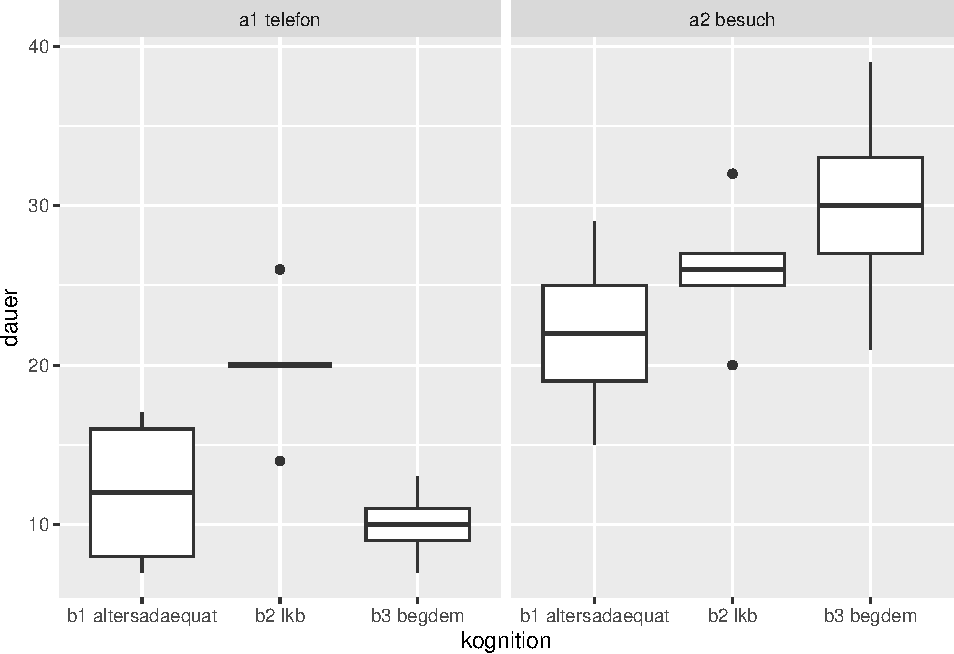
\includegraphics{desc_aov_files/figure-latex/aboxplot-1.pdf}
\caption{\label{fig:aboxplot}Boxplots of all combinations of \texttt{modus} and \texttt{kognition}}
\end{figure}

\clearpage

\hypertarget{interaction-plots}{%
\section{Interaction Plots}\label{interaction-plots}}

\begin{figure}
\centering
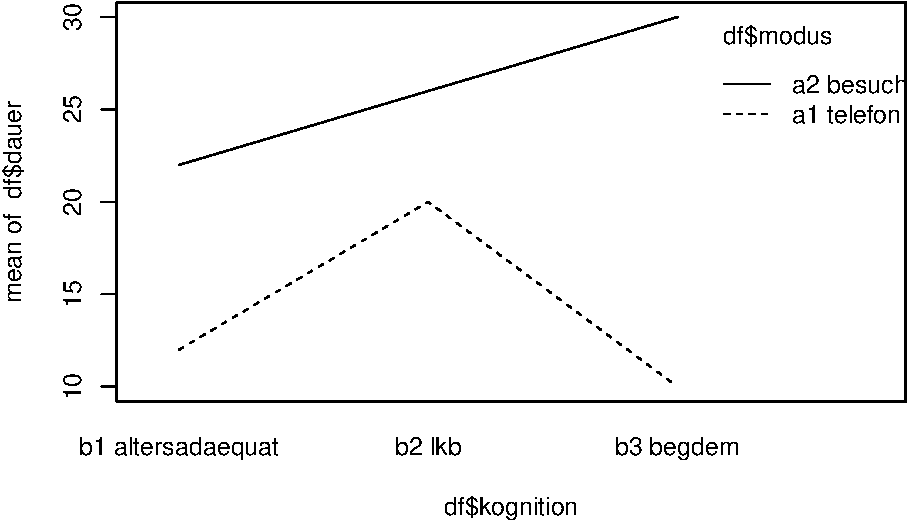
\includegraphics{desc_aov_files/figure-latex/iplotdauerkog-1.pdf}
\caption{\label{fig:iplotdauerkog}Interaction Plot: \texttt{dauer} and \texttt{modus}}
\end{figure}

\begin{figure}
\centering
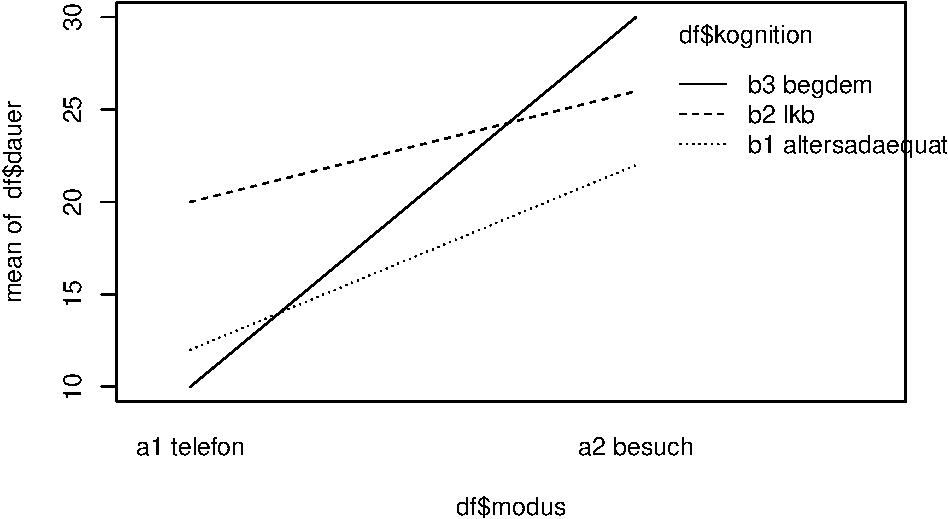
\includegraphics{desc_aov_files/figure-latex/iplotdauermod-1.pdf}
\caption{\label{fig:iplotdauermod}Interaction Plot: \texttt{dauer} and \texttt{kognition}}
\end{figure}

\begin{table}[tbp]

\begin{center}
\begin{threeparttable}

\caption{\label{tab:tabanova}A beautiful ANOVA table.}

\begin{tabular}{lllllll}
\toprule
Effect & \multicolumn{1}{c}{$\hat{\eta}^2_G$} & \multicolumn{1}{c}{90\% CI} & \multicolumn{1}{c}{$F$} & \multicolumn{1}{c}{$\mathit{df}$} & \multicolumn{1}{c}{$\mathit{df}_{\mathrm{res}}$} & \multicolumn{1}{c}{$p$}\\
\midrule
Modus & .665 & {}[.462, .778] & 47.65 & 1 & 24 & < .001\\
Kognition & .249 & {}[.014, .450] & 3.97 & 2 & 24 & .032\\
Modus $\times$ Kognition & .323 & {}[.062, .517] & 5.74 & 2 & 24 & .009\\
\bottomrule
\addlinespace
\end{tabular}

\begin{tablenotes}[para]
\normalsize{\textit{Anmerkungen.} Bli bla blubb.}
\end{tablenotes}

\end{threeparttable}
\end{center}

\end{table}

\hypertarget{contrast-matrix}{%
\section{Contrast Matrix}\label{contrast-matrix}}

\begin{Shaded}
\begin{Highlighting}[]
\FunctionTok{contrasts}\NormalTok{(df}\SpecialCharTok{$}\NormalTok{kognition) }\OtherTok{\textless{}{-}} \FunctionTok{cbind}\NormalTok{(}\FunctionTok{c}\NormalTok{(}\DecValTok{2}\NormalTok{, }\SpecialCharTok{{-}}\DecValTok{1}\NormalTok{, }\SpecialCharTok{{-}}\DecValTok{1}\NormalTok{), }\FunctionTok{c}\NormalTok{(}\DecValTok{0}\NormalTok{, }\DecValTok{1}\NormalTok{,}\SpecialCharTok{{-}}\DecValTok{1}\NormalTok{)) }
\end{Highlighting}
\end{Shaded}

\begin{table}[tbp]

\begin{center}
\begin{threeparttable}

\caption{\label{tab:tabanovaext}A beautiful ANOVA table.}

\begin{tabular}{lllllll}
\toprule
Effect & \multicolumn{1}{c}{$\hat{\eta}^2_G$} & \multicolumn{1}{c}{90\% CI} & \multicolumn{1}{c}{$F$} & \multicolumn{1}{c}{$\mathit{df}$} & \multicolumn{1}{c}{$\mathit{df}_{\mathrm{res}}$} & \multicolumn{1}{c}{$p$}\\
\midrule
Modus & .665 & {}[.462, .778] & 47.65 & 1 & 24 & < .001\\
Kognition & .249 & {}[.014, .450] & 3.97 & 2 & 24 & .032\\
Kognition $\times$  altersadäquat vs beeinträchtigt & .199 & {}[.018, .419] & 5.96 & 1 & 24 & .022\\
Kognition $\times$  LKB vs beginnende Demenz & .076 & {}[.000, .282] & 1.99 & 1 & 24 & .172\\
Modus $\times$ Kognition & .323 & {}[.062, .517] & 5.74 & 2 & 24 & .009\\
Modus $\times$ Kognition $\times$  altersadäquat vs beeinträchtigt & .199 & {}[.018, .419] & 5.96 & 1 & 24 & .022\\
Modus $\times$ Kognition $\times$  LKB vs beginnende Demenz & .187 & {}[.013, .407] & 5.51 & 1 & 24 & .027\\
\bottomrule
\addlinespace
\end{tabular}

\begin{tablenotes}[para]
\normalsize{\textit{Anmerkungen.} Bli bla blubb.}
\end{tablenotes}

\end{threeparttable}
\end{center}

\end{table}

\hypertarget{data-modkogdat3f.csv}{%
\section{\texorpdfstring{Data \texttt{ModKogDat3F.csv}}{Data ModKogDat3F.csv}}\label{data-modkogdat3f.csv}}

\begin{Shaded}
\begin{Highlighting}[]
\NormalTok{df3 }\OtherTok{\textless{}{-}} \FunctionTok{read.csv}\NormalTok{(}\StringTok{"../data/ModKogDat3F.csv"}\NormalTok{, }\AttributeTok{header=}\ConstantTok{TRUE}\NormalTok{, }\AttributeTok{sep=}\StringTok{","}\NormalTok{) }\SpecialCharTok{|\textgreater{}} 
  \FunctionTok{mutate}\NormalTok{(}
    \AttributeTok{modus =} \FunctionTok{as.factor}\NormalTok{(modus),}
    \AttributeTok{kognition =} \FunctionTok{as.factor}\NormalTok{(kognition),}
    \AttributeTok{interviewer =} \FunctionTok{as.factor}\NormalTok{(interviewer)}
\NormalTok{  ) }\SpecialCharTok{|\textgreater{}} 
    \FunctionTok{group\_by}\NormalTok{(modus, kognition, interviewer) }\SpecialCharTok{|\textgreater{}} 
  \FunctionTok{mutate}\NormalTok{(}
    \AttributeTok{id\_num =} \FunctionTok{cur\_group\_id}\NormalTok{(),}
    \AttributeTok{m\_str =} \FunctionTok{substr}\NormalTok{(modus, }\DecValTok{1}\NormalTok{, }\DecValTok{2}\NormalTok{),}
    \AttributeTok{k\_str =} \FunctionTok{substr}\NormalTok{(kognition, }\DecValTok{1}\NormalTok{, }\DecValTok{2}\NormalTok{),}
    \AttributeTok{i\_str =} \FunctionTok{substr}\NormalTok{(interviewer, }\DecValTok{1}\NormalTok{, }\DecValTok{2}\NormalTok{),}
    \AttributeTok{id =} \FunctionTok{paste}\NormalTok{(m\_str, k\_str, i\_str, }\AttributeTok{sep =} \StringTok{"\_"}\NormalTok{)}
\NormalTok{  ) }\SpecialCharTok{|\textgreater{}} 
  \FunctionTok{select}\NormalTok{(}\SpecialCharTok{{-}}\NormalTok{m\_str, }\SpecialCharTok{{-}}\NormalTok{k\_str, }\SpecialCharTok{{-}}\NormalTok{i\_str) }\SpecialCharTok{|\textgreater{}} 
  \FunctionTok{tibble}\NormalTok{() }
\end{Highlighting}
\end{Shaded}

\begin{table}[tbp]

\begin{center}
\begin{threeparttable}

\caption{\label{tab:tabinspect3}Full Dataset: `ModKogDat3F.csv`}

\begin{tabular}{llllll}
\toprule
dauer & \multicolumn{1}{c}{modus} & \multicolumn{1}{c}{kognition} & \multicolumn{1}{c}{interviewer} & \multicolumn{1}{c}{id\_num} & \multicolumn{1}{c}{id}\\
\midrule
8 & telefon & altersadaequat & ehrenamt & 7 & te\_al\_eh\\
16 & telefon & altersadaequat & ehrenamt & 7 & te\_al\_eh\\
12 & telefon & altersadaequat & ehrenamt & 7 & te\_al\_eh\\
7 & telefon & altersadaequat & ehrenamt & 7 & te\_al\_eh\\
17 & telefon & altersadaequat & ehrenamt & 7 & te\_al\_eh\\
20 & telefon & lkb & ehrenamt & 11 & te\_lk\_eh\\
26 & telefon & lkb & ehrenamt & 11 & te\_lk\_eh\\
20 & telefon & lkb & ehrenamt & 11 & te\_lk\_eh\\
14 & telefon & lkb & ehrenamt & 11 & te\_lk\_eh\\
20 & telefon & lkb & ehrenamt & 11 & te\_lk\_eh\\
10 & telefon & begdem & ehrenamt & 9 & te\_be\_eh\\
7 & telefon & begdem & ehrenamt & 9 & te\_be\_eh\\
11 & telefon & begdem & ehrenamt & 9 & te\_be\_eh\\
9 & telefon & begdem & ehrenamt & 9 & te\_be\_eh\\
13 & telefon & begdem & ehrenamt & 9 & te\_be\_eh\\
15 & hausbesuch & altersadaequat & ehrenamt & 1 & ha\_al\_eh\\
25 & hausbesuch & altersadaequat & ehrenamt & 1 & ha\_al\_eh\\
22 & hausbesuch & altersadaequat & ehrenamt & 1 & ha\_al\_eh\\
19 & hausbesuch & altersadaequat & ehrenamt & 1 & ha\_al\_eh\\
29 & hausbesuch & altersadaequat & ehrenamt & 1 & ha\_al\_eh\\
32 & hausbesuch & lkb & ehrenamt & 5 & ha\_lk\_eh\\
27 & hausbesuch & lkb & ehrenamt & 5 & ha\_lk\_eh\\
26 & hausbesuch & lkb & ehrenamt & 5 & ha\_lk\_eh\\
20 & hausbesuch & lkb & ehrenamt & 5 & ha\_lk\_eh\\
25 & hausbesuch & lkb & ehrenamt & 5 & ha\_lk\_eh\\
30 & hausbesuch & begdem & ehrenamt & 3 & ha\_be\_eh\\
21 & hausbesuch & begdem & ehrenamt & 3 & ha\_be\_eh\\
33 & hausbesuch & begdem & ehrenamt & 3 & ha\_be\_eh\\
39 & hausbesuch & begdem & ehrenamt & 3 & ha\_be\_eh\\
27 & hausbesuch & begdem & ehrenamt & 3 & ha\_be\_eh\\
8 & telefon & altersadaequat & profi & 8 & te\_al\_pr\\
16 & telefon & altersadaequat & profi & 8 & te\_al\_pr\\
12 & telefon & altersadaequat & profi & 8 & te\_al\_pr\\
7 & telefon & altersadaequat & profi & 8 & te\_al\_pr\\
17 & telefon & altersadaequat & profi & 8 & te\_al\_pr\\
20 & telefon & lkb & profi & 12 & te\_lk\_pr\\
26 & telefon & lkb & profi & 12 & te\_lk\_pr\\
20 & telefon & lkb & profi & 12 & te\_lk\_pr\\
14 & telefon & lkb & profi & 12 & te\_lk\_pr\\
20 & telefon & lkb & profi & 12 & te\_lk\_pr\\
10 & telefon & begdem & profi & 10 & te\_be\_pr\\
7 & telefon & begdem & profi & 10 & te\_be\_pr\\
11 & telefon & begdem & profi & 10 & te\_be\_pr\\
9 & telefon & begdem & profi & 10 & te\_be\_pr\\
13 & telefon & begdem & profi & 10 & te\_be\_pr\\
15 & hausbesuch & altersadaequat & profi & 2 & ha\_al\_pr\\
25 & hausbesuch & altersadaequat & profi & 2 & ha\_al\_pr\\
22 & hausbesuch & altersadaequat & profi & 2 & ha\_al\_pr\\
19 & hausbesuch & altersadaequat & profi & 2 & ha\_al\_pr\\
29 & hausbesuch & altersadaequat & profi & 2 & ha\_al\_pr\\
32 & hausbesuch & lkb & profi & 6 & ha\_lk\_pr\\
27 & hausbesuch & lkb & profi & 6 & ha\_lk\_pr\\
26 & hausbesuch & lkb & profi & 6 & ha\_lk\_pr\\
20 & hausbesuch & lkb & profi & 6 & ha\_lk\_pr\\
25 & hausbesuch & lkb & profi & 6 & ha\_lk\_pr\\
30 & hausbesuch & begdem & profi & 4 & ha\_be\_pr\\
21 & hausbesuch & begdem & profi & 4 & ha\_be\_pr\\
33 & hausbesuch & begdem & profi & 4 & ha\_be\_pr\\
39 & hausbesuch & begdem & profi & 4 & ha\_be\_pr\\
27 & hausbesuch & begdem & profi & 4 & ha\_be\_pr\\
\bottomrule
\end{tabular}

\end{threeparttable}
\end{center}

\end{table}

\begin{table}[tbp]

\begin{center}
\begin{threeparttable}

\caption{\label{tab:tabsumstat3}Summary Statistics: `ModKogDat3F.csv`}

\begin{tabular}{llllllll}
\toprule
Variables & \multicolumn{1}{c}{n} & \multicolumn{1}{c}{mean} & \multicolumn{1}{c}{sd} & \multicolumn{1}{c}{median} & \multicolumn{1}{c}{min} & \multicolumn{1}{c}{max} & \multicolumn{1}{c}{se}\\
\midrule
dauer & 30.00 & 20.00 & 8.44 & 20.00 & 7.00 & 39.00 & 1.54\\
modus* & 30.00 & 1.50 & 0.51 & 1.50 & 1.00 & 2.00 & 0.09\\
kognition* & 30.00 & 2.00 & 0.83 & 2.00 & 1.00 & 3.00 & 0.15\\
id\_num & 30.00 & 3.50 & 1.74 & 3.50 & 1.00 & 6.00 & 0.32\\
id* & 30.00 & 3.50 & 1.74 & 3.50 & 1.00 & 6.00 & 0.32\\
\bottomrule
\addlinespace
\end{tabular}

\begin{tablenotes}[para]
\normalsize{\textit{Anmerkungen.} This table contains all variables.}
\end{tablenotes}

\end{threeparttable}
\end{center}

\end{table}

\begin{table}[tbp]

\begin{center}
\begin{threeparttable}

\caption{\label{tab:tabsummary3}Summary Statistics for the Variable `dauer`:  `ModKogDat3F.csv`}

\begin{tabular}{llllllllll}
\toprule
id & \multicolumn{1}{c}{count} & \multicolumn{1}{c}{mean} & \multicolumn{1}{c}{sd} & \multicolumn{1}{c}{COV (sd/mean)} & \multicolumn{1}{c}{min} & \multicolumn{1}{c}{q25} & \multicolumn{1}{c}{median} & \multicolumn{1}{c}{q75} & \multicolumn{1}{c}{max}\\
\midrule
ha\_al\_eh & 5 & 22.00 & 5.39 & 0.24 & 15 & 19.00 & 22 & 25.00 & 29\\
ha\_al\_pr & 5 & 22.00 & 5.39 & 0.24 & 15 & 19.00 & 22 & 25.00 & 29\\
ha\_be\_eh & 5 & 30.00 & 6.71 & 0.22 & 21 & 27.00 & 30 & 33.00 & 39\\
ha\_be\_pr & 5 & 30.00 & 6.71 & 0.22 & 21 & 27.00 & 30 & 33.00 & 39\\
ha\_lk\_eh & 5 & 26.00 & 4.30 & 0.17 & 20 & 25.00 & 26 & 27.00 & 32\\
ha\_lk\_pr & 5 & 26.00 & 4.30 & 0.17 & 20 & 25.00 & 26 & 27.00 & 32\\
te\_al\_eh & 5 & 12.00 & 4.53 & 0.38 & 7 & 8.00 & 12 & 16.00 & 17\\
te\_al\_pr & 5 & 12.00 & 4.53 & 0.38 & 7 & 8.00 & 12 & 16.00 & 17\\
te\_be\_eh & 5 & 10.00 & 2.24 & 0.22 & 7 & 9.00 & 10 & 11.00 & 13\\
te\_be\_pr & 5 & 10.00 & 2.24 & 0.22 & 7 & 9.00 & 10 & 11.00 & 13\\
te\_lk\_eh & 5 & 20.00 & 4.24 & 0.21 & 14 & 20.00 & 20 & 20.00 & 26\\
te\_lk\_pr & 5 & 20.00 & 4.24 & 0.21 & 14 & 20.00 & 20 & 20.00 & 26\\
\bottomrule
\addlinespace
\end{tabular}

\begin{tablenotes}[para]
\normalsize{\textit{Anmerkungen.} This table contains summary statistics for each combination of `modus`,  `kognition`, and `interviewer`}
\end{tablenotes}

\end{threeparttable}
\end{center}

\end{table}

\begin{figure}
\centering
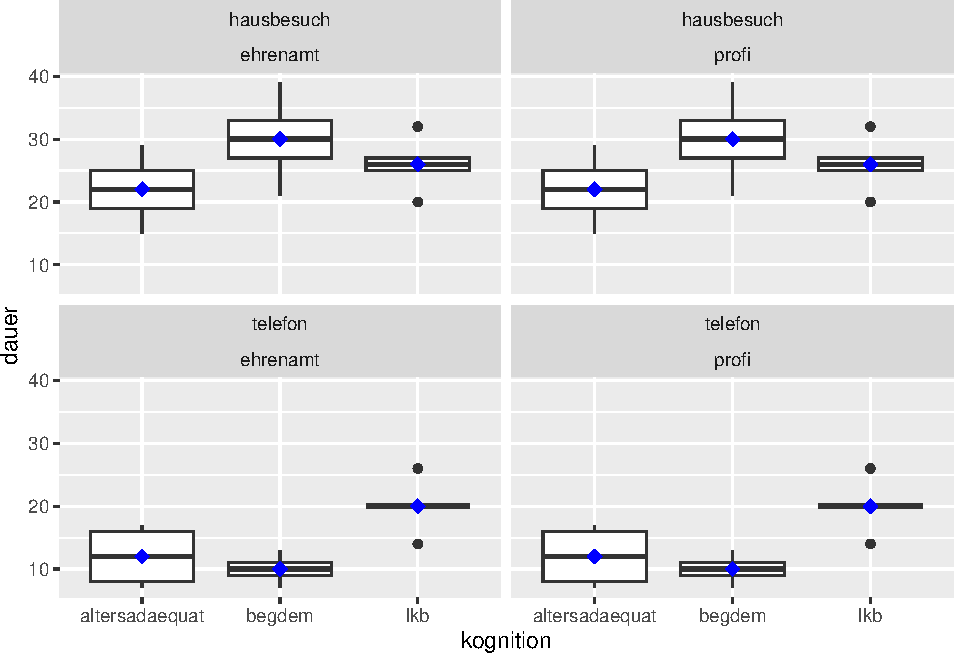
\includegraphics{desc_aov_files/figure-latex/df3boxplot-1.pdf}
\caption{\label{fig:df3boxplot}Boxplots of all combinations of \texttt{modus}, \texttt{kognition}, and \texttt{interviewer}}
\end{figure}

\begin{table}[tbp]

\begin{center}
\begin{threeparttable}

\caption{\label{tab:tabanova3}A beautiful ANOVA table with `interviewer`.}

\begin{tabular}{lllllll}
\toprule
Effect & \multicolumn{1}{c}{$\hat{\eta}^2_G$} & \multicolumn{1}{c}{90\% CI} & \multicolumn{1}{c}{$F$} & \multicolumn{1}{c}{$\mathit{df}$} & \multicolumn{1}{c}{$\mathit{df}_{\mathrm{res}}$} & \multicolumn{1}{c}{$p$}\\
\midrule
Modus & .665 & {}[.533, .751] & 95.29 & 1 & 48 & < .001\\
Kognition & .249 & {}[.077, .398] & 7.94 & 2 & 48 & .001\\
Interviewer & .000 & {}[.000, .000] & 0.00 & 1 & 48 & > .999\\
Modus $\times$ Kognition & .323 & {}[.140, .469] & 11.47 & 2 & 48 & < .001\\
Modus $\times$ Interviewer & .000 & {}[.000, .000] & 0.00 & 1 & 48 & > .999\\
Kognition $\times$ Interviewer & .000 & {}[.000, .000] & 0.00 & 2 & 48 & > .999\\
Modus $\times$ Kognition $\times$ Interviewer & .000 & {}[.000, .000] & 0.00 & 2 & 48 & > .999\\
\bottomrule
\addlinespace
\end{tabular}

\begin{tablenotes}[para]
\normalsize{\textit{Anmerkungen.} Bli bla blubb.}
\end{tablenotes}

\end{threeparttable}
\end{center}

\end{table}

\newpage

\hypertarget{excercises}{%
\section{Excercises}\label{excercises}}

\begin{enumerate}
\def\labelenumi{\arabic{enumi}.}
\tightlist
\item
  In Table \ref{tab:tabsumstat3} is an error. What is wrong here? Please correct.
\item
  Table \ref{tab:tabinspect3} is too long. Please split it up to two tables by interviewer.
\item
  Tables that relate to \texttt{ModKogDat3F.csv} data are not yet mentioned in the summary. Please add them, because, according to APA rules, each Figure and Table, respectively, must be mentioned in the text.
\end{enumerate}

\newpage

\hypertarget{solutions}{%
\section{Solutions}\label{solutions}}

\begin{enumerate}
\def\labelenumi{\arabic{enumi}.}
\tightlist
\item
  The wrong dataframe was used here. The correct data is \texttt{df3}. Table \ref{tab:tabsumstat3correct} is the correct one.
\end{enumerate}

\begin{Shaded}
\begin{Highlighting}[]
\NormalTok{tabsumstat3 }\OtherTok{\textless{}{-}}\NormalTok{ df3 }\SpecialCharTok{|\textgreater{}}
\NormalTok{  psych}\SpecialCharTok{::}\FunctionTok{describe}\NormalTok{()   }\SpecialCharTok{|\textgreater{}} 
  \FunctionTok{as\_tibble}\NormalTok{(}\AttributeTok{rownames=}\StringTok{"Variables"}\NormalTok{)  }\SpecialCharTok{|\textgreater{}} 
  \FunctionTok{select}\NormalTok{(}\SpecialCharTok{{-}}\NormalTok{skew, }\SpecialCharTok{{-}}\NormalTok{kurtosis, }\SpecialCharTok{{-}}\NormalTok{range, }\SpecialCharTok{{-}}\NormalTok{vars, }\SpecialCharTok{{-}}\NormalTok{trimmed, }\SpecialCharTok{{-}}\NormalTok{mad) }

\FunctionTok{apa\_table}\NormalTok{(}
\NormalTok{  tabsumstat3}
\NormalTok{  , }\AttributeTok{caption =} \StringTok{"Summary Statistics: \textasciigrave{}ModKogDat3F.csv\textasciigrave{}"}
\NormalTok{  , }\AttributeTok{note =} \StringTok{"This table contains all variables."}
\NormalTok{  , }\AttributeTok{escape =} \ConstantTok{TRUE}
\NormalTok{)}
\end{Highlighting}
\end{Shaded}

\begin{table}[tbp]

\begin{center}
\begin{threeparttable}

\caption{\label{tab:tabsumstat3correct}Summary Statistics: `ModKogDat3F.csv`}

\begin{tabular}{llllllll}
\toprule
Variables & \multicolumn{1}{c}{n} & \multicolumn{1}{c}{mean} & \multicolumn{1}{c}{sd} & \multicolumn{1}{c}{median} & \multicolumn{1}{c}{min} & \multicolumn{1}{c}{max} & \multicolumn{1}{c}{se}\\
\midrule
dauer & 60.00 & 20.00 & 8.36 & 20.00 & 7.00 & 39.00 & 1.08\\
modus* & 60.00 & 1.50 & 0.50 & 1.50 & 1.00 & 2.00 & 0.07\\
kognition* & 60.00 & 2.00 & 0.82 & 2.00 & 1.00 & 3.00 & 0.11\\
interviewer* & 60.00 & 1.50 & 0.50 & 1.50 & 1.00 & 2.00 & 0.07\\
id\_num & 60.00 & 6.50 & 3.48 & 6.50 & 1.00 & 12.00 & 0.45\\
id* & 60.00 & 6.50 & 3.48 & 6.50 & 1.00 & 12.00 & 0.45\\
\bottomrule
\addlinespace
\end{tabular}

\begin{tablenotes}[para]
\normalsize{\textit{Anmerkungen.} This table contains all variables.}
\end{tablenotes}

\end{threeparttable}
\end{center}

\end{table}

\begin{enumerate}
\def\labelenumi{\arabic{enumi}.}
\setcounter{enumi}{1}
\tightlist
\item
  The splitted tables are shown in Tables \ref{tab:tabinspect3p} and \ref{tab:tabinspect3e} and here is the corresponding code:
\end{enumerate}

\begin{Shaded}
\begin{Highlighting}[]
\NormalTok{df3p }\OtherTok{\textless{}{-}}\NormalTok{ df3 }\SpecialCharTok{|\textgreater{}} 
  \FunctionTok{filter}\NormalTok{(interviewer }\SpecialCharTok{==} \StringTok{"profi"}\NormalTok{)}
\NormalTok{df3e }\OtherTok{\textless{}{-}}\NormalTok{ df3 }\SpecialCharTok{|\textgreater{}} 
  \FunctionTok{filter}\NormalTok{(interviewer }\SpecialCharTok{==} \StringTok{"ehrenamt"}\NormalTok{)}
\end{Highlighting}
\end{Shaded}

\begin{Shaded}
\begin{Highlighting}[]
\FunctionTok{apa\_table}\NormalTok{(df3p,  }\AttributeTok{caption =} \StringTok{"Interviews by Professionals"}\NormalTok{)}
\end{Highlighting}
\end{Shaded}

\begin{table}[tbp]

\begin{center}
\begin{threeparttable}

\caption{\label{tab:tabinspect3p}Interviews by Professionals}

\begin{tabular}{llllll}
\toprule
dauer & \multicolumn{1}{c}{modus} & \multicolumn{1}{c}{kognition} & \multicolumn{1}{c}{interviewer} & \multicolumn{1}{c}{id\_num} & \multicolumn{1}{c}{id}\\
\midrule
8 & telefon & altersadaequat & profi & 8 & te\_al\_pr\\
16 & telefon & altersadaequat & profi & 8 & te\_al\_pr\\
12 & telefon & altersadaequat & profi & 8 & te\_al\_pr\\
7 & telefon & altersadaequat & profi & 8 & te\_al\_pr\\
17 & telefon & altersadaequat & profi & 8 & te\_al\_pr\\
20 & telefon & lkb & profi & 12 & te\_lk\_pr\\
26 & telefon & lkb & profi & 12 & te\_lk\_pr\\
20 & telefon & lkb & profi & 12 & te\_lk\_pr\\
14 & telefon & lkb & profi & 12 & te\_lk\_pr\\
20 & telefon & lkb & profi & 12 & te\_lk\_pr\\
10 & telefon & begdem & profi & 10 & te\_be\_pr\\
7 & telefon & begdem & profi & 10 & te\_be\_pr\\
11 & telefon & begdem & profi & 10 & te\_be\_pr\\
9 & telefon & begdem & profi & 10 & te\_be\_pr\\
13 & telefon & begdem & profi & 10 & te\_be\_pr\\
15 & hausbesuch & altersadaequat & profi & 2 & ha\_al\_pr\\
25 & hausbesuch & altersadaequat & profi & 2 & ha\_al\_pr\\
22 & hausbesuch & altersadaequat & profi & 2 & ha\_al\_pr\\
19 & hausbesuch & altersadaequat & profi & 2 & ha\_al\_pr\\
29 & hausbesuch & altersadaequat & profi & 2 & ha\_al\_pr\\
32 & hausbesuch & lkb & profi & 6 & ha\_lk\_pr\\
27 & hausbesuch & lkb & profi & 6 & ha\_lk\_pr\\
26 & hausbesuch & lkb & profi & 6 & ha\_lk\_pr\\
20 & hausbesuch & lkb & profi & 6 & ha\_lk\_pr\\
25 & hausbesuch & lkb & profi & 6 & ha\_lk\_pr\\
30 & hausbesuch & begdem & profi & 4 & ha\_be\_pr\\
21 & hausbesuch & begdem & profi & 4 & ha\_be\_pr\\
33 & hausbesuch & begdem & profi & 4 & ha\_be\_pr\\
39 & hausbesuch & begdem & profi & 4 & ha\_be\_pr\\
27 & hausbesuch & begdem & profi & 4 & ha\_be\_pr\\
\bottomrule
\end{tabular}

\end{threeparttable}
\end{center}

\end{table}

\begin{Shaded}
\begin{Highlighting}[]
\FunctionTok{apa\_table}\NormalTok{(df3e,  }\AttributeTok{caption =} \StringTok{"Interviews by Volunteers (Ehrenamt)"}\NormalTok{)}
\end{Highlighting}
\end{Shaded}

\begin{table}[tbp]

\begin{center}
\begin{threeparttable}

\caption{\label{tab:tabinspect3e}Interviews by Volunteers (Ehrenamt)}

\begin{tabular}{llllll}
\toprule
dauer & \multicolumn{1}{c}{modus} & \multicolumn{1}{c}{kognition} & \multicolumn{1}{c}{interviewer} & \multicolumn{1}{c}{id\_num} & \multicolumn{1}{c}{id}\\
\midrule
8 & telefon & altersadaequat & ehrenamt & 7 & te\_al\_eh\\
16 & telefon & altersadaequat & ehrenamt & 7 & te\_al\_eh\\
12 & telefon & altersadaequat & ehrenamt & 7 & te\_al\_eh\\
7 & telefon & altersadaequat & ehrenamt & 7 & te\_al\_eh\\
17 & telefon & altersadaequat & ehrenamt & 7 & te\_al\_eh\\
20 & telefon & lkb & ehrenamt & 11 & te\_lk\_eh\\
26 & telefon & lkb & ehrenamt & 11 & te\_lk\_eh\\
20 & telefon & lkb & ehrenamt & 11 & te\_lk\_eh\\
14 & telefon & lkb & ehrenamt & 11 & te\_lk\_eh\\
20 & telefon & lkb & ehrenamt & 11 & te\_lk\_eh\\
10 & telefon & begdem & ehrenamt & 9 & te\_be\_eh\\
7 & telefon & begdem & ehrenamt & 9 & te\_be\_eh\\
11 & telefon & begdem & ehrenamt & 9 & te\_be\_eh\\
9 & telefon & begdem & ehrenamt & 9 & te\_be\_eh\\
13 & telefon & begdem & ehrenamt & 9 & te\_be\_eh\\
15 & hausbesuch & altersadaequat & ehrenamt & 1 & ha\_al\_eh\\
25 & hausbesuch & altersadaequat & ehrenamt & 1 & ha\_al\_eh\\
22 & hausbesuch & altersadaequat & ehrenamt & 1 & ha\_al\_eh\\
19 & hausbesuch & altersadaequat & ehrenamt & 1 & ha\_al\_eh\\
29 & hausbesuch & altersadaequat & ehrenamt & 1 & ha\_al\_eh\\
32 & hausbesuch & lkb & ehrenamt & 5 & ha\_lk\_eh\\
27 & hausbesuch & lkb & ehrenamt & 5 & ha\_lk\_eh\\
26 & hausbesuch & lkb & ehrenamt & 5 & ha\_lk\_eh\\
20 & hausbesuch & lkb & ehrenamt & 5 & ha\_lk\_eh\\
25 & hausbesuch & lkb & ehrenamt & 5 & ha\_lk\_eh\\
30 & hausbesuch & begdem & ehrenamt & 3 & ha\_be\_eh\\
21 & hausbesuch & begdem & ehrenamt & 3 & ha\_be\_eh\\
33 & hausbesuch & begdem & ehrenamt & 3 & ha\_be\_eh\\
39 & hausbesuch & begdem & ehrenamt & 3 & ha\_be\_eh\\
27 & hausbesuch & begdem & ehrenamt & 3 & ha\_be\_eh\\
\bottomrule
\end{tabular}

\end{threeparttable}
\end{center}

\end{table}

\begin{enumerate}
\def\labelenumi{\arabic{enumi}.}
\setcounter{enumi}{2}
\tightlist
\item
  The unmentioned tables are Tables \ref{tab:tabinspect3}, \ref{tab:tabsumstat3}, \ref{tab:tabsummary3}, \ref{tab:tabanova3}, and Figure \ref{fig:df3boxplot}.
\end{enumerate}

\newpage

\hypertarget{references}{%
\section*{References}\label{references}}
\addcontentsline{toc}{section}{References}

\hypertarget{refs}{}
\begin{CSLReferences}{1}{0}
\leavevmode\vadjust pre{\hypertarget{ref-R-papaja}{}}%
Aust, F., \& Barth, M. (2023). \emph{{papaja}: {Prepare} reproducible {APA} journal articles with {R} markdown}. Retrieved from \url{https://github.com/crsh/papaja}

\end{CSLReferences}


\clearpage
\renewcommand{\listfigurename}{Figure captions}

\clearpage
\renewcommand{\listtablename}{Table captions}


\end{document}
